\documentclass[a4paper,12pt,oneside,CJK]{cctbook}

\textwidth  = 16cm
\textheight = 24cm
\topmargin  = -6mm
\oddsidemargin  = 30pt
\evensidemargin = 30pt
\baselineskip = 20mm
\renewcommand{\baselinestretch}{1.5}

%\usepackage{cite}
\usepackage{amsmath,amssymb,amsthm}
%\usepackage{empheq}   %-------to use \empheq
\usepackage{titlesec}
%\usepackage{algorithm,algorithmic}
\usepackage{graphicx,subfigure}
\usepackage{epstopdf}
%\usepackage{multirow}
%\usepackage[colorlinks=true,linkcolor=blue,citecolor=green]{hyperref}

\DeclareGraphicsRule{jpg}{eps}{bb}{}
%\allowdisplaybreaks

\newtheorem{thm}  {\indent 定理}[section]
\newtheorem{cor}  {\indent 推论}[section]
\newtheorem{lem}  {\indent 引理}[section]
\newtheorem{prop} {\indent 命题}[section]
\newtheorem{assum}{\indent 假设}[section]
\newtheorem{propn}{\indent 性质}[section]

\renewcommand{\proofname}{\bf 证明}

\theoremstyle{definition}
\newtheorem{prob} {\indent 问题}[section]
\newtheorem{defn} {\indent 定义}[section]
\newtheorem{rem}  {\indent 注}  [section]

\numberwithin{equation}{section}
\renewcommand{\theequation}{\thesection.\arabic{equation}}
%\renewcommand{\thefigure}  {\thesection.\arabic{figure}}

\renewcommand{\thefootnote}{\fnsymbol{footnote}}
\newpagestyle{main}[\small]{
\sethead{\kaishu\chaptername\quad\chaptertitle}{}{\kaishu\sectionname\quad\sectiontitle}
\setfoot{}{\thepage}{}
\headrule
}

\begin{document}


% 封一
\pagestyle{empty}

\begin{flushright}
{\zihao{-4}
学校代码:10246{\ \ \ \ \ \ \ \ \ \ \ }\\
学{\hspace{18pt}}号:12110180019
}
\end{flushright}
\vspace{4mm}

\begin{center}
%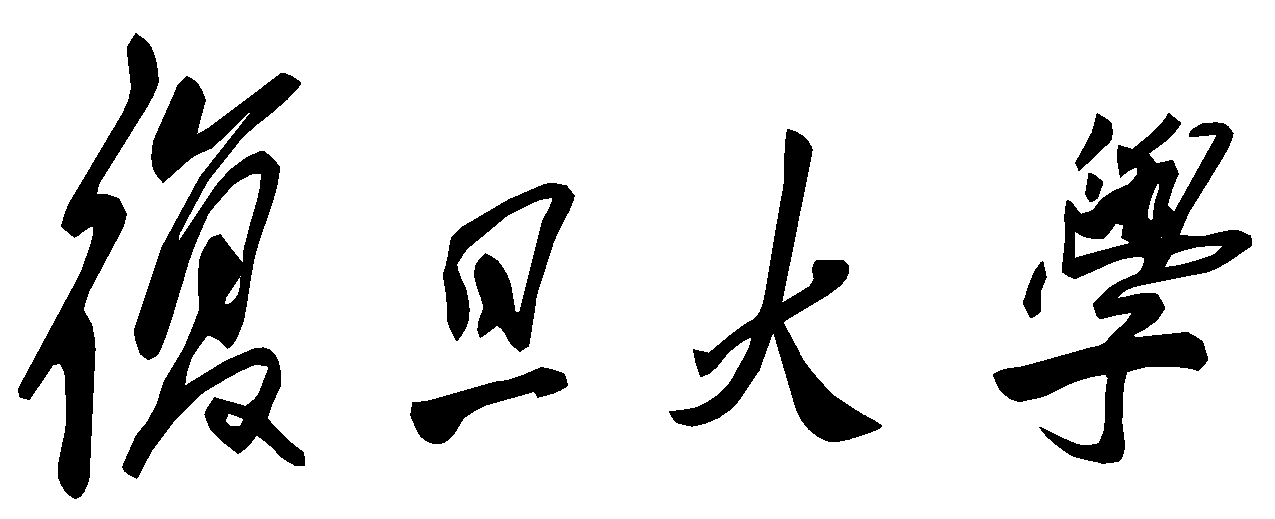
\includegraphics[width=0.6\textwidth]{fig/FudanLogo.eps}
\end{center}
\vspace{4mm}

\begin{center}
{\zihao{2}
硕\quad 士\quad 学\quad 位\quad 论\quad 文
}\\
\vspace{2.5cm}
{\zihao{2}
{\heiti {\LARGE\bf 地下水模型渗透率参数的反演}}
}\\
\vspace{1cm}
{\Large
empty
}
\end{center}
\vspace{2cm}

\begin{center}
{\zihao{4}
院{\hspace{39pt}}系: \underline{\qquad 数\ 学\ 科\ 学\ 学\ 院 \qquad }\\
\vspace{4mm}
专{\hspace{39pt}}业: \underline{\qquad\quad 计\ 算\ 数\ 学 \qquad\qquad }\\
\vspace{4mm}
姓{\hspace{39pt}}名: \underline{\qquad\qquad 钱\ 浩\qquad\qquad\ \ }\\
\vspace{4mm}
指\ 导\ 教\ 师: \underline{\qquad\quad 程\ 晋\ \ \ 教\ 授 \quad\qquad\ }\\
\vspace{4mm}
完\ 成\ 日\ 期: \underline{\qquad\quad 2015\ 年\ 03\ 月 \quad\qquad\ }
}
\end{center}


% 扉页
\newpage
\thispagestyle{empty}

\begin{center}
{\zihao{3}
{\heiti 指\ 导\ 教\ 师:}\\
\vspace{1cm}
{程\ 晋\ \ \ 教\ 授}\\
\vspace{2cm}
{\heiti  指\ 导\ 小\ 组\ 成\ 员:}\\
\vspace{1cm}
{程\ 晋\ \ \ 教\ 授}\\
\vspace{4mm}
{陆\ 帅\ \ \ 副\ 研\ 究\ 员}
}
\end{center}


% 目录
\newpage
\pagestyle{plain}
\frontmatter
\tableofcontents


% 中文摘要
\newpage
\pagestyle{plain}
\mainmatter

\addcontentsline{toc}{chapter}{\heiti 中文摘要}

\centerline{\zihao{3}\heiti{\large\bf DA}空}
\vspace{6mm}

\centerline{\zihao{3}\heiti 摘\ \ \ \ 要}
\vspace{2mm}

ddd
\\
{\bf 关键词:} 非线性反问题,迭代正则化方法,数据同化,贝叶斯方法,滤波,地下水模型。\\
{\bf 中图分类号:}\quad O29。


% 英文摘要
\newpage

\addcontentsline{toc}{chapter}{\bf Abstract}

\centerline{\large\bf empty}
\vspace{6mm}

\centerline{\bf\large Abstract}
\vspace{2mm}

ddd
\\
{\bf Keywords: }  nonlinear inverse problems, iterative regularization, data assimilation,  Bayesian inversion, filtering method, groundwater model.\\
{\bf Chinese Library Classification: }\quad O29.

% ---- 正文 ---- %

\newpage
\pagestyle{main}



\chapter{引言及预备知识}\label{chp:intro}
本章首先介绍本文中主要研究的地下水模型、非线性反问题及其正则化方法等概念,同时也将进一步引入Bayesian统计方法量化反演地下水模型渗透率过程中的不确定性。

\section{反问题}
反问题一般随着正问题成对出现,由于历史的原因,其中一类问题被人们研究得比较透彻。一般来说,可以称此类问题为正问题(direct~problems)。
例如,给定一个偏微分方程及其参数、求解区域、初边值条件,求解方程的过程一般都是一个正问题。
然而,当确定某些数学模型中未知参数来解释观测数据、现象的时候,
反问题(inverse~problem)往往就会随之产生。
反问题在天文学、大气海洋学、医学、量子力学等应用领域中广泛存在。
较为常见的反问题往往考虑的是反演数学模型中的变量参数,
这些参数往往具有极为重要的物理意义,但很难直接测量。
比如,上述偏微分方程问题的方程未知参数、初值或者边值中的某些条件是未知的,
那么就需要通过其他附加的可测量信息来确定这些未知的参数。
在实际的生产生活中,
越来越多的反问题被提出来,
而这些问题都亟待解决。
为了解决实际生产生活当中遇到的困难,
对于反问题或者不适定问题的研究变得十分的重要。

从数学上来看,反问题的形式往往可以表现为以下的抽象算子方程:
\begin{eqnarray*}
    y=\mathcal{G}(u),
\end{eqnarray*}
其中$u\in X$,$y\in Y$,$X$和$Y$均为Banach空间或Hilbert空间,
$y$是我们的观测数据,而$u$是我们希望反演得到的真解或参数,
$\mathcal{G}$一般被称为正问题算子,在本文中,作者将主要关注非线性形式的椭圆方程正问题。

当针对实际问题建立相应的数学模型之后,我们首先要考虑
正问题提法的合理性,也就是Hadamard提出的适定性研究。
数学上的适定性定义是指以下三点
\begin{enumerate}
   \item 存在性:问题的解是存在的;
  \item 唯一性:问题的解是唯一的;
  \item 稳定性:问题的解连续依赖于给定数据。
\end{enumerate}
如果上述某一个条件不能得到满足,
则称这样的问题是不适定的。前文提到的正、反问题中,一般有一个问题是不适定的,人们往往将其称为反问题。可以认为,我们研究的反问题都是不适定的。

在数学上,对于解的存在性,
可以用扩大求解空间来找到合适的解。
如果问题存在多个的解,
可以通过增加限制条件筛选出符合要求的解。
问题的稳定性是应用中比较看重的一点,
实际生产或实验中获取的数据基本上都是测量数据,
由于测量仪器的精度、人为操作等原因,测量数据难免会出现测量误差。
而稳定性要求数据上小的误差只会引起问题解的小扰动。
因此能否保证问题解的稳定性在应用中显得极为重要。


\section{Landweber迭代正则化方法}

对于具有不适定性的反问题,人们往往利用正则化方法来实现稳定的反演。常用的正则化方法有Tikhonov正则化和
Landweber迭代正则化。而在求解非线性反问题的时候,Landweber非线性正则化方法较为常用。下文将给出正则化方法的简单定义,并针对线性、非线性反问题探讨Landweber迭代的格式。

首先介绍一下线性问题的正则化方法的定义。假定$K:X\rightarrow Y$是线性紧算子,对精确的右端数据$y$,方程
$$Kx=y$$
存在唯一解$x$.设有误差的右端数据$y^{\delta}$满足
\begin{align}\label{eq1_operator}
Kx=y^{\delta} = y + \delta\eta
\end{align}
其中,$\delta$为误差界,也即$\|y^{\delta}-y\|\leq \delta$,$\eta$是满足一定分布的噪音,例如确定性框架下的均匀分布噪音。

对于一般的线性问题,可以给出如下的正则化方法定义
\begin{defn}\label{def1_regularization}[正则化方法]
一族有界线性算子$R_{\alpha}:Y\rightarrow X, \alpha>0$
称为线性算子方程(\ref{eq1_operator})的正则化算子,若存在一个参数选取准则$\alpha=\alpha(y^{\delta},\delta)$,使得成立
\begin{align*}
\lim_{\delta\rightarrow 0}\sup\{\|R_{\alpha(y^{\delta},\delta)} y^{\delta} - x^{\dag}\| \, |\, y^{\delta}\in Y, \|y^{\delta}-y\|\leq \delta \} & = 0 \\
\lim_{\delta\rightarrow 0}\sup\{\alpha(y^{\delta},\delta) \, | \, y^{\delta}, \|y^{\delta}-y\|\leq \delta \} & = 0
\end{align*}
对所有的$x\in X$成立,这里的$\alpha$称为正则化参数。
\end{defn}

由定义\ref{def1_regularization},成立如下性质:
\begin{enumerate}
   \item 对任一固定的$\alpha>0$,$R_{\alpha}$是有界的;
  \item 在$X$上,$\alpha\rightarrow 0$时$R_{\alpha}K$逐点收敛于单位算子$I$;
  \item 该定义等价于$R_{\alpha}y\rightarrow K^{-1}y$对一切的$y\in K(X)$成立。
\end{enumerate}
对于非线性问题而言,其定义也类似,这里省去这部分内容。

对于线性问题(\ref{eq1_operator}),一个直接求解方法就是最小二乘法,也即找到$x_{LS}$成立
\begin{align}\label{eq1_lsquare}
x_{LS} = \min_{x\in X}\{\frac{1}{2}\|Kx - y\|^2\}.
\end{align}
但是由于反问题的不适定性,最小二乘法在噪音数据下的应用非常有限。

Landweber迭代算法就是从最小二乘法衍生而来的一类正则化方法,譬如带噪音的情况下,最小二乘法(\ref{eq1_lsquare})的Euler方程直接给出了以下的关系
\begin{align*}
K^*(Kx-y^{\delta}) = 0.
\end{align*}
取一个松弛因子$a>0$,我们把上式改写成为
$$
    x=(I-a K^*K)x+a K^*y^{\delta},
$$
并用迭代法求解此方程,即得到了线性反问题的Landweber迭代格式
$$
    x^0=0,\qquad x^m=(I-a K^* K)x^{m-1}+a K^*y,~m=1,2,3\cdots
$$
事实上,$x^m=x^{m-1}-a K^*(K x^{m-1}-y)$可以看成是以步长为$a$的最速下降迭代序列。
同时,可以将$x^m$显式表示为$x_m=R_m y,$算子$R_m:Y\rightarrow X$为
\begin{eqnarray*}
   R_m\equiv a\sum_{k=0}^{m-1}(I-a K^* K)^k K^*,~m=1,2,3,\cdots,
\end{eqnarray*}
定义\ref{def1_regularization}中的正则化参数变为$\alpha=1/m$. 选取合适的停机准则,譬如残差法则(Discrepancy principle),可以得到稳定的反演。

非线性问题$y^{\delta}=\mathcal{G}(u)$的Landweber迭代法也可以看成是最小二乘法的衍生品,按上节内容,可以直接给出非线性问题的Landweber迭代格式
$$
    x^0=0,\qquad x^m=x^{m-1}-a \mathcal{G}'^*(\mathcal{G}(x^{m-1})-y^{\delta}),~m=1,2,3\cdots
$$
其中$\mathcal{G}'^*$是非线性正问题算子线性化后的伴随算子。同样的,在本文中,停机准则为残差法则,也即迭代次数$m_{DP}$满足
\begin{align}\label{eq1_DP}
\|\mathcal{G}(x_{m_{DP+1}}) - y^{\delta}\| \leq C \delta \leq \|\mathcal{G}(x_{m_{DP}}) - y^{\delta}\|
\end{align}
这里的常数$C>1$.

事实上,Landweber迭代正则化方法的形式可以拓展到其他正则化方法或数值方法。例如,
通过迭代预条件的方法把$K(x)=y^{\delta}$化为
\begin{eqnarray*}
   B(n,x)(K(x)-y^{\delta})=0,n\in N
\end{eqnarray*}
其中$B(n,x):Y\rightarrow X$是线性有界算子,因此迭代格式变为
\begin{eqnarray*}
   x_{n+1}=x_n-B(n,x_n)(K(x_n)-y^{\delta}).
\end{eqnarray*}
若取$B(n,x)=K'(x)^{-1}$,则得到Newton迭代格式;取$B(n,x) = (K'^*(x)K'+\alpha I )^{-1} K'^*$则得到Levenberg-Marquardt方法等,这里就不一一详细说明。

\section{贝叶斯方法}
前章提到的正则化方法是确定性框架下的反问题求解方法,一般只能处理均匀分布或一致有界的噪音。如果噪音是Gaussian分布的白噪音,那么之前的确定性方法无法使用。反问题领域中,最常用的用于解决一般噪音反问题的统计方法是贝叶斯方法。在贝叶斯方法里,无论是真解还是噪音,
都用随机量来表示,两者均被描述为某种独立的概率分布。更一般而言,贝叶斯方法反演得到的结果不再是前章正则化方法提供的一个逼近解,而是提供了先验讯息的目标参数在观测值下的后验概率分布。

在贝叶斯方法的框架下,我们考虑一类特殊的有限维的向量方程,也即(\ref{eq1_operator})变为
\begin{eqnarray*}
    y=\mathcal{G}(u)+\eta, \quad u\in \mathbb{R}^n,\, y\in \mathbb{R}^m
\end{eqnarray*}
其中$\eta$是Gaussian白噪声,满足分布$\mathcal{N}(0,\Gamma)$,其中$\Gamma\in R^{m\times m}$。而真解$u$也是满足Gaussian分布且独立于$\eta$的随机变量,满足先验分布$\mathcal{N}(m_0,C_0)$,其中$m_0 \in R^n$及$C_0\in R^{n\times n}$.
贝叶斯方法来源于著名的贝叶斯公式:
\begin{eqnarray*}
    \pi(u|y^{\delta})=\frac{\pi(u,y^{\delta})}{\pi(y^{\delta})}=\frac{\pi(y^{\delta}|u)\pi(u)}{\pi(y^{\delta})},
\end{eqnarray*}
其中$\pi(u)$为先验分布,$\pi(u,y^{\delta})$是联合分布,$\pi(y^{\delta}|u)$是条件分布(一般称为似然函数),$\pi(u|y^{\delta})$为我们关心的后验分布。在应用贝叶斯方法的时候,更加常用的形式是
\begin{align}\label{eq1_bayes}
    \pi(u|y^{\delta}) \propto \pi(y^{\delta}|u)\pi(u),
\end{align}
也即后验分布正比于似然函数乘以先验分布。

贝叶斯方法的研究一般集中在构造后验分布$\pi(u|y^{\delta})$,并以此提取感兴趣的统计反演解。例如,最常用的一个统计反演解是最大后验估计(Maximum a posteriori (MAP) estimate),也即寻找(假设存在的)$u_{MAP}$,使得后验概率密度函数得到最大值,i.e.
\begin{align*}
u_{MAP}=\arg\max_{u\in \mathbb{R}^n} \pi(u|y).
\end{align*}
注意到这里的最大后验估计不一定唯一。在Gaussian框架下,最大后验估计满足的泛函等价于确定性框架下的Tikhonov正则化,我们将在后文中进一步展开。另外一个点态的统计反演解是条件期望(Conditional mean (CM)),也即在以下积分收敛的意义下的统计反演解$x_{CM}$
\begin{align*}
u_{CM} = \mathbb{E}\{u|y^{\delta}\} = \int_{\mathbb{R}^n} u \pi(u|y^{\delta}) dx.
\end{align*}
条件期望的解定义在一个积分之上,所以在求解过程中需要讨论该(高维)积分的计算,我们将在后文中专门讨论针对的采样算法。

为了得到后验分布$\pi(u|y^{\delta})$,我们因此需要提供似然函数$\pi(y^{\delta}|u)$以及先验分布$\pi(u)$。在构造似然函数的过程中,我们可以充分利用噪音的分布讯息。例如,在有限维中考虑Gaussian白噪音$\mathcal{N}(0,\Gamma)$,那么条件分布$\pi(y^{\delta}|u)=\mathcal{N}(\mathcal{G}(u),\Gamma)$,并且其密度函数$\rho(y^{\delta|u})$满足
\begin{align*}
\rho(y^{\delta}|u): = \textrm{exp}\left(-\frac{1}{2}\|y^{\delta}-\mathcal{G}(u)\|_{\Gamma}^2\right)
\end{align*}
其中$\|\cdot\|_{\Gamma}^2 = \|\Gamma^{-1/2}\cdot\|$满足我们提出的噪音模型。结合先验分布$\mathcal{N}(m_0,C_0)$,就得到了后验密度函数
\begin{align*}
\rho(u|y^{\delta}) \propto \textrm{exp}\left(-\frac{1}{2}\|y^{\delta}-\mathcal{G}(u)\|_{\Gamma}^2-\frac{1}{2}\|u-m_0\|_{C_0}^2\right).
\end{align*}
显然,之前提到的MAP估计就等价于求解
\begin{align*}
u_{MAP} = \arg\min_{u\in R^n} \frac{1}{2}\|y^{\delta}-\mathcal{G}(u)\|_{\Gamma}^2+\frac{1}{2}\|u-m_0\|_{C_0}^2
\end{align*}
也即确定性意义下的Tikhonov正则化方法。


有限维Bayesian方法的后验分布可以通过贝叶斯公式直接给出,与其不同的是,无限维的函数空间Bayesian方法需要验证其后验分布的适定性。这就需要介绍一下函数空间意义下的贝叶斯定理。不妨假设正问题算子$\mathcal{G}:X\rightarrow Y$是作用在可分Banach空间$X$和$Y$上的映射,方程形式同(\ref{eq1_operator}),但
$\eta\sim \mathbb{Q}_0,u \sim \mu_0$,且分布$\mathbb{Q}_0$和$\mu_0$独立。进一步定义$X\times Y$上的乘积测度
\begin{eqnarray*}
    \nu_0(du,dy)&=&\mu_0(du)  \otimes Q_0(dy)
\end{eqnarray*}
我们由此给出以下广义的贝叶斯定理
\begin{thm}\label{thm_bayesian}
假定映射$\mathcal{G}: X \times Y \rightarrow R$是$\nu_0$可测,且满足
\begin{align*}
y^{\delta} = \mathcal{G}u + \eta.
\end{align*}
若$y^{\delta}$对于$\mathbb{Q}_0$几乎处处可测,并且
$$Z:=\int_X \exp(-\Phi(u;y))\mu_0 (du)>0.$$
那么条件分布$u|y^{\delta}$在$\nu$下存在,我们将其表示为$\mu^y$。更进一步, 如果$\mu^y \ll \mu_0$且$y^{\delta}$对于$\mathbb{Q}_0$几乎处处可测,则成立
$$\frac{d\mu^y}{d\mu_0}(u)=\frac{1}{Z}\exp\left(-\Phi(u;y)\right).$$
\end{thm}















若要使用贝叶斯定理,需满足如下4个条件:
\begin{enumerate}
\item 先验测度$\mu_0$与噪声测度$Q_0$是在测度$\nu_0$意义下是独立的
\item $\Phi$的关系式能够成立.
\item 证明$\Phi$是$\nu_0$可测的。
\item 证明常数$Z$几乎处处大于0。
\end{enumerate}

\begin{assum}\label{ass1}
 令$X'\in X$ 并假定$\Phi\in C(X'\times Y;R)$在闭集上是
Lipschitz的,进一步有函数$M_i:R^+\times R^+\rightarrow R^+,~i=1,2$,为单调非减函数,
且$M_2$严格大于0,对于所有的$u\in X'$,$y_1,y_2,y\in B_Y(0,r)$,成立
\begin{eqnarray*}
   \Phi(u,y)&\geq& -M_1(r,||u||_X),\\
   |\Phi(u,y_1)-\Phi(u,y_2)|&\leq& M_2(r,||u||_X)||y_1-y_2||_Y.
\end{eqnarray*}
\end{assum}

\begin{thm}
若假设\ref{ass1}成立,假设$\mu_0(X')=1$且存在闭集$B\in X$使得
$\mu_0(X'\cap B)>0$,那么则有对于任意的$y\in Y$都有$Z(y)>0,$ 并且$\mu^y$是适定的。
\end{thm}

\subsection{贝叶斯方法的稳定性}

对于贝叶斯方法的稳定性,我们首先引入Hellinger距离,再给出关于稳定性的定理。

令$\mu$和$\mu'$是两个概率测度,在$R^l$上分别拥有严格正的概率密度$\rho$和$\rho'$。

定义$\rho$和$\rho'$的Hellinger距离如下:
\begin{eqnarray*}
    d_{Hell}(\mu,\mu ')&=&\sqrt{\frac{1}{2}\int_{R^l}(1-\sqrt{\frac{\rho'(x)}{\rho(x)}})^2\rho(x)dx}\\
    &=&(\frac{1}{2}E^{\mu}(1-\sqrt{\frac{\rho'(x)}{\rho(x)}}^2))^{\frac{1}{2}}
\end{eqnarray*}

\begin{thm} 若假设\ref{ass1}成立,并假设$\mu_0(X')=1$且存在闭集$B\in X$使得
$\mu_0(X'\cap B)>0$,更进一步若对于每一个固定的$r>0$,满足
$$\exp(M_1(r,||u||_X))(1+M_2^2(r,||u||_X))\in L_{\mu_0}^1(X;R)$$.
那么则存在$C=C(r)$,使得对于任意的$y,y'\in B_Y(0,r)$
\begin{eqnarray*}
   d_{Hell}(\mu^y,\mu^{y'})\leq C ||y-y'||_Y
\end{eqnarray*}
\end{thm}

\section{数据同化}

数据同化方法建立在贝叶斯方法上的基础之上,
贝叶斯方法考虑的情况往往是观测数据已经全部采集,
而数据同化方法则可以不断加入新的观测数据,
将原有观测值和新观测值结合,求解后验分布$u|y$。
相比于贝叶斯方法,数据同化方法所需要的观测数据更少,
在地下水问题、石油分布等问题中更具有应用价值。

\subsection{数据同化的定义}

令映射$\Psi:R^n\rightarrow R^n$,考虑如下动力系统:
\begin{eqnarray*}
    u_{j+1}&=&\Psi(u_j), j\in N\\
    u_0&\sim& N(m_0,C_0).
\end{eqnarray*}
其中$m_0$和$C_0$为常数.我们的目标就是通过该系统的$\{u_j\}$求解计算获得初值$u_0.$
然而在实际的应用中,我们往往只能得到一些测量值,不能得到$u=\{u_j\}_{j\in Z^+}$.
因此我们往往得到的是$u_j$的观测值,并带有噪声:
\begin{eqnarray*}
  y_{j+1}=h(u_{j+1})+\eta_{j+1},j\in N
\end{eqnarray*}
其中$h:R^n\rightarrow R^m$,$\eta=\{\eta_j\}$是独立同分布的序列,且与$u$无关。

对于过程中的每一步,可看成贝叶斯方法的运用,
因此我们有如下定理。

\textbf{Theorem} 对于如上的确定性动力系统来说,
记后验分布$v_0|y$的概率密度为$\mu$,$y={y_j}_{j=1}^J$
即$P(u_0|y)=\mu(u)$,满足$\mu(u)\propto \exp(-I_0(u_0;y))$,其中
\begin{eqnarray*}
   I_0(u_0;y)&=&J_0(u_0)+\Phi_0(u_0;y),\\
   J_0(u_0)&=&\frac{1}{2}|C_0^{-\frac{1}{2}}(u_0-m_0)|^2,\\
   \Phi_0(u_0;y)&=&\sum_{j=0}^{J-1}\frac{1}{2}|\Gamma^{-\frac{1}{2}}(y_{j+1}-h(\Psi^{(j+1)}(u_0)))|^2.
\end{eqnarray*}

\subsection{更新过程}

数据同化的更新过程:
我们令$Y_j=\{y_l\}_{l=1}^j,$
通过$P(u_{j}|Y_j)$计算得到$P(u_{j+1}|Y_{j+1})$,
一般分为两步:
\begin{enumerate}
  \item 预测:$P(u_{j}|Y_j)\rightarrow P(u_{j+1}|Y_j)$;
  \item 分析:$P(u_{j+1}|Y_j)\rightarrow P(u_{j+1}|Y_{j+1})$;
\end{enumerate}

第一步预测,易得
\begin{eqnarray*}
   P(u_{j+1}|Y_j)&=&\int_{R^{n}}P(u_{j+1}|Y_j,u_j)P(u_j)du_j\\
                 &=&\int_{R^{n}}P(u_{j+1}|u_j)P(u_j|Y_j)du_j\\
\end{eqnarray*}
$P(u_{j+1}|u_j)$是可以,从而确定$P(u_{j+1}|Y_j)$,
积分式即是映射$\Psi$与$P(u_{j}|Y_j)$作卷积,可记作$\Psi \star P(u_j|Y_j)$

第二步分析,利用贝叶斯公式得
\begin{eqnarray*}
     P(u_{j+1}|Y_{j+1})&=&P(u_{j+1}|Y_j,y_{j+1})\\
    &=&\frac{P(y_{j+1}|u_{j+1},Y_j)P(u_{j+1}|Y_j)}{P(y_{j+1}|Y_j)}\\
    &=&\frac{P(y_{j+1}|u_{j+1})P(u_{j+1}|Y_j)}{P(y_{j+1}|Y_j)}.
\end{eqnarray*}
从而实现$P(u_{j+1}|Y_j)\rightarrow P(u_{j+1}|Y_{j+1})$

\subsection{适定性}

下面我们考察解的适定性。
令$\mu_0$为确定性动力系统中$v_0$的先验测度,
$\mu$和$\mu'$是两个来自不同观察数据$y$和$y'$所得的后验测度。
下面的定理将给出的结论是:在Hellinger距离的意义下,
后验测度对于观察数据是连续依赖的,且是Lipschitz连续的。

\textbf{Theorem}
考虑由确定性动力系统产生的后验分布,
如有$$E^{\mu_0}(\sum_{j=0}^{J-1}1+|h(\Psi^{(j+1)}(v_0))|^2)^{\frac{1}{2}}< \infty$$,
那么,对于$|y|,|y'|\leq r$,存在常数$c=c(r)$使得
$$d_{HEll}(\mu,\mu')\leq c(r)|y-y'|.$$









\section{地下水模型}
本文中,我们将考虑如下的区域$D\in R^d$,$\partial D$为其Lipschitz边界。
定义Hilbert空间为$V\subset H \subset V*$,其中$V = H_0^1(D)$, $H=L^2(D)$。
本文讨论的地下水模型基于Darcy定律,并有如下的二阶椭圆方程形式
\begin{align}\label{eq1_groundwater}
\left\{
\begin{array}{rl}
    -\nabla\cdot(K\nabla p)=f,  & \quad in\quad D\\
     p=0, & \quad on \quad \partial D
\end{array}
\right.
\end{align}
其中$f\in V^*$,渗透率$K\in X^+ = \{v\in L^{\infty}(D)|{\rm ess} \inf_{x\in D} v(x) = \kappa_{\min}>0\}$。我们讨论的正问题为映射$\mathcal{G}:X^+\rightarrow V$,且满足
$$\mathcal{G}(K)=p,$$
也即将渗透率映射成可观测的水压$p$。根据二阶椭圆方程理论,(\ref{eq1_groundwater})存在唯一的弱解,且有$\|p\|_V \leq \|f\|_{V^*}/\kappa_{\min}$。事实上$\mathcal{G}(\cdot)$算子是一个有界算子,且满足
\begin{lem}\label{lem_groundwater}
对于$i=1,2$,
\begin{eqnarray*}
   -\nabla\cdot(K_i\nabla p_i)&=&f \quad in\quad D\\
     p_i&=&0\quad on \quad \partial D
\end{eqnarray*}
则有
$$\|p_1-p_2\|_V\leq \frac{1}{K_{\min}^2}\|f\|_{V^*}\|K_1-K_2\|_{L^{\infty}}$$
这里取
$$K_{\min}:={\rm ess} \inf_{x\in D}K_1(x)\wedge {\rm ess} \inf_{x\in D}K_2(x)>0.$$
\end{lem}

地下水渗透率表现的是地下的水文结构,并在石油工业中有着重要的应用。事实上,地下水渗透率研究的应用前景包括了的注入并保存温室气体。通过对于地层结构的渗透率反演,得到地下近似地貌及水文结构,从而可以确定低渗透率地层内部区域作为温室气体的储存层,减少泄露的危险。对于这里应用的进一步讨论,可参考...


\chapter{Landweber正则化方法反演地下水渗透率}
在本章中,我们利用确定性框架下的Landweber非线性迭代正则化方法实现地下水渗透率的反演。Landweber非线性迭代的过程中,需要涉及以下抽象算子的推断。
\section{线性化算子}
事实上,为了保证Landweber非线性迭代正则化方法的有效实施,我们需要首先证明正问题算子是Fr\'{e}chet可导。对于上章提到的地下水模型(\ref{eq1_groundwater}),
我们建立正问题映射$\mathcal{G}$,满足$\mathcal{G}:X^+\rightarrow Y$,满足
\begin{eqnarray}
   \mathcal{G}(K)=p.
\end{eqnarray}

我们首先验证$\mathcal{G}$算子的Gateaux导数形式。
\begin{thm}\label{thm2_Fderi}~令$i=1,2$,$K_i\in X^+,$并且$K_2=K_1+\epsilon h,h\in X^+,||h||_{\infty}=1,$
满足地下水模型(\ref{eq1_groundwater}),且有$\mathcal{G}(K_i) = p_i$。则非线性算子$\mathcal{G}$在$K_1$处Gateaux可导,且导数$\mathcal{G}' h : h \rightarrow u$,这里令$u:=\lim_{\epsilon\rightarrow 0}\frac{p_2-p_1}{\epsilon}$且满足如下方程
\begin{align}\label{eq2_Fderi}
    -\nabla\cdot(K_1\nabla u)&=\nabla\cdot(h\nabla p_1) \quad in\quad D\\
     u&=0\quad on \quad \partial D.
\end{align}
\end{thm}

\textbf{证明}

由已知条件,$K_1,K_2$满足
\begin{eqnarray*}
   -\nabla\cdot(K_i\nabla p_i)&=&f \quad in~D\\
   p_i&=&0\quad on ~\partial D
\end{eqnarray*}
两式相减可得
\begin{eqnarray*}
   -\nabla\cdot((K_1-K_2)\nabla p_1)-\nabla\cdot(K_2\nabla (p_1-p_2))&= & 0 \quad in~D \\
   p_1-p_2& = & 0 \quad on ~\partial D.
\end{eqnarray*}
两式左右两端同除以$\epsilon$并令$\epsilon\rightarrow 0$,整理后即得
\begin{eqnarray*}
    -\nabla\cdot(K_1\nabla u)&=&\nabla\cdot(h\nabla p_1) \quad in\quad D\\
     u&=&0\quad on \quad \partial D.
\end{eqnarray*}

我们进一步证明,定理\ref{thm2_Fderi}中的Gateaux导数$\mathcal{G}'(\cdot)$事实上是正问题算子$\mathcal{G}$的Fr\'{e}chet导数,也即证明
\begin{eqnarray}
   \|p_2-p_1- u\|_V\sim o(\|h\|_{L^{\infty}}),
\end{eqnarray}
这里$K_2 = K_1 + h$,且$p_i  = \mathcal{G}(K_i)$,$i=1,2$。则我们可以首先得到
\begin{align*}
-\nabla\cdot (K_1 \nabla (p_2-p_1)) & = \nabla\cdot (h\nabla p_2), \quad in ~D \\
p_2-p_1 & = 0,\quad on ~\partial D,
\end{align*}
由引理\ref{lem_groundwater}可知存在一个一般的常数$c$,使得成立
\begin{align}\label{eq2_p2minusp1}
\|p_2-p_1\|_{V} \leq c \|\nabla\cdot( h\nabla p_2)\|_{V^*} \leq c \|h\|_{L^{\infty}} \|p_2\|_{V}.
\end{align}
又由已知条件,$K_1,K_2$满足
\begin{eqnarray*}
   -\nabla\cdot(K_i\nabla p_i)&=&f \quad in~D\\
   p_i&=&0\quad on ~\partial D.
\end{eqnarray*}
线性化形式中的$u$满足
\begin{eqnarray*}
    -\nabla\cdot(K_1\nabla u)&=&\nabla(h\nabla p_1) \quad in\quad D\\
     u&=&0\quad on \quad \partial D.
\end{eqnarray*}
那么我们定义$v = p_1-p_2- u$,可得
\begin{eqnarray*}
   -\nabla\cdot(K_2\nabla p_2-K_1\nabla (p_1+ u))&=&\nabla\cdot(h\nabla p_1) \quad in~D\\
   p_2-p_1-u&=&0\quad on ~\partial D
\end{eqnarray*}
所以根据引理\ref{lem_groundwater},我们有如下估计式
\begin{eqnarray*}
    \|v\|_V \leq \epsilon ^2 \|\nabla\cdot(h\nabla (p_1-p_2))\|_{V^*}\\
\end{eqnarray*}
结合(\ref{eq2_p2minusp1})可得
\begin{eqnarray*}
   \|v\|_{V} \leq c \|h\|_{L^{\infty}} \|p_1-p_2\|_V \leq c \|h\|_{L^{\infty}}^2 \sim o(\|h\|_{L^{\infty}})
\end{eqnarray*}
这样就证明了我们所求的Gateaux导数$\mathcal{G}'(\cdot)$即为算子$\mathcal{G}$的Fr\'{e}chet导数,即如下定理
\begin{thm}\label{thm2_Fderi2}~令非线性算子$\mathcal{G}$
满足地下水模型(\ref{eq1_groundwater}),且有$\mathcal{G}(K) = p$。则该算子在$K$处Fr\'{e}chet可导,该导数$\mathcal{G}' : X^+ \rightarrow Y$,且$\forall h\in X^+$满足如下方程
\begin{align*}
    -\nabla\cdot(K\nabla u)&=\nabla\cdot(h\nabla p) \quad in\quad D\\
     u&=0\quad on \quad \partial D.
\end{align*}
\end{thm}

\section{伴随算子}
在Landweber迭代正则化方法中,我们需要进一步计算正问题线性化后的伴随算子,也即$\mathcal{G'}^*$。这里,我们采用的方法是最优控制中的Lagrange乘子法。首先,构造Lagrange泛函
\begin{align*}
\mathcal{L}(p,K,q)&=\frac{1}{2}\int_D (p-p_m)^2 d x-\int_D(-\nabla\cdot (K\nabla p)-f)q d x
\end{align*}
这里的$q$是我们的Lagrange乘子。由分部积分可得
\begin{eqnarray*}
   \mathcal{L}(p,K,q)&=&\frac{1}{2}\int_D (p-p_m)^2 d x-\int_D(-\nabla\cdot (K\nabla p)-f)q d x\\
              &=&\frac{1}{2}\int_D (p-p_m)^2 d x+\int_D(\nabla\cdot (K\nabla q) p+f q) d x\\
&-&\int_{\partial D} K\frac{\partial q}{\partial \nu} p~dx +\int_{\partial D} K\frac{\partial p}{\partial \nu}q~dx.
\end{eqnarray*}
对Lagrange乘子取$\ell$方向的$p$-Gateaux导数,也即
\begin{eqnarray}\label{eq-DF*}
    \mathcal{L}_p(p,K,q)l&=&\int_D (p-p_m) \ell dx+\int_D(\nabla\cdot (K\nabla q)\ell d x\\
&-&\int_{\partial D} K\frac{\partial q}{\partial \nu}\ell dx +\int_{\partial D} K \frac{\partial \ell}{\partial \nu}qdx
\end{eqnarray}
其中,测试函数$\ell\in C_0^{\infty}$。不妨取在边界$\partial D$上$\ell(x)=0$及$\frac{\partial \ell}{\partial\nu}=0$,因此可得伴随算子满足的方程
\begin{align*}
   -\nabla\cdot(K\nabla q)&=p-p_m\quad in~D.
\end{align*}
再取测试函数在边界$\partial D$上满足$\ell(x)=0$,则可得伴随算子的边界条件
\begin{align*}
   q=0\quad on~ \partial D.
\end{align*}
因此,我们得到了以下的伴随算子形式

\begin{thm}\label{thm2_Fadjoint}~令非线性算子$\mathcal{G}$
满足地下水模型(\ref{eq1_groundwater}),且有$\mathcal{G}(K) = p$。则该算子的伴随为$\mathcal{G'}^* : Y \rightarrow X^+$,且满足如下方程
\begin{align}\label{eq2_Fadjoint}
   -\nabla\cdot(K\nabla q)&=p-p_m \quad in~ D\\
     q&=0\quad on~ \partial D.
\end{align}
\end{thm}

结合(\ref{eq1_groundwater})和(\ref{eq2_Fadjoint}),我们就得到Landweber迭代正则化方法为
\begin{eqnarray}\label{eq-DF*s}
    K_{j+1}=K_j-\mu \mathcal{G'}(K_j)^*(\mathcal{G}(K_j)-p_m), \quad j=1,2\ldots,
\end{eqnarray}
这里的$p_m$是观测数据.


\section{算法及算例}

在这一部分我们将运用Landeweber迭代公式\ref{eq-DF*s}
反演地下水模型的渗透率参数$K$.

正问题的算法我们采用经典的有限元算法。我们通过$\kappa=\log(K)$来设定真解
$K^{\dagger}$。区域$D=[0,1]\times[0,1]$,$f=1~in~D$,算例模型如下
\begin{eqnarray*}
    -\nabla\cdot(K\nabla P)&=&1 \quad in\quad [0,1]\times [0,1]\\
     P&=&0\quad on \quad x=0,y=1,x=1,y=0
\end{eqnarray*}
我们取
\begin{eqnarray}
   \kappa^{\dagger}=randn(x,y), (x,y)\in [0,1]\times [0,1],
\end{eqnarray}
回忆反问题算子为
\begin{eqnarray}
   \mathcal{G}(K)=p
\end{eqnarray}
噪音$\xi$添加到观测值$p$上,且满足$\xi~N(0,1)$,有如下形式
\begin{eqnarray*}
   p^{\gamma}=p+\gamma \xi
\end{eqnarray*}
其中常数$\gamma$表示为噪音的等级,我们设定它为$10^{-3}$

考虑到问题的不适定性,我们需要设置一个合理的停止准则。
在无噪音的情况下,我们设定的停止准则为
\begin{eqnarray}
   \frac{||K_{i+1}-K_i||}{||K_i||}\leq 10^{-5}
\end{eqnarray}

计算的初始值取$\kappa_0=1.05\times\kappa^{\dagger}$。
图\ref{fig1}的左边显示的是真解$K^{\dagger}$,右边显示的是迭代停止时的计算解$K_{593},$
满足停止准则。图\ref{fig2}的左边显示的是迭代过程中残差$||\mathcal{G}(K_i)-p||~,i=1,\cdots,593$在对数尺度下的情况,
右边显示的是计算解与真解的相对误差$\frac{||K_i-K^{\dagger}||}{||K^{\dagger}||},~i=1,\cdots,593$在对数尺度下的情况.

从计算的结果来看,随着迭代次数的增加,残差与相对误差逐步下降。当迭代步数达到593步、
迭代停止的时候,相对误差$\frac{||K_{593}-K^{\dagger}||}{||K^{\dagger}||}\approx 0.0158$。
实际上,我们可以通过选择更小的停止准则增加迭代步数,从而提高计算精度,
但是也会导致计算量增加。

\begin{figure}
\subfigure[$K^{\dagger}$]{
\centering
\includegraphics[width=0.4\textwidth]{L-true.eps}%
}
\subfigure[$K_{593}$]{
\centering
\includegraphics[width=0.4\textwidth]{L-s.eps}
}
\caption{图左显示的是真解$K^{\dagger}$,图右显示的是迭代停止时的计算解$K_{593}$}\label{fig1}
\end{figure}

\begin{figure}
\subfigure[Residual]{
\centering
\includegraphics[width=0.4\textwidth]{L-r.eps}%
}
\subfigure[Solution error]{
\centering
\includegraphics[width=0.4\textwidth]{L-s-e.eps}
}
\caption{图左显示的是迭代过程中残差$||\mathcal{G}(K_i)-p||)~,i=1,\cdots,593$在对数尺度下的情况,
图右显示的是计算解与真解的相对误差$\frac{||K_i-K^{\dagger}||}{||K^{\dagger}||},~i=1,\cdots,593$在对数尺度下的情况}\label{fig2}
\end{figure}

在有噪音的情况下,根据偏差原理,我们设定的停止准则为
\begin{eqnarray}
   ||p^{\gamma}-F(K_{j^*})||\leq \tau \gamma < ||p^{\gamma}-F(K_j)||~0\leq j<j^*
\end{eqnarray}
其中$\tau\geq 1$,

计算的初始值取$\kappa_0=1.01\times\kappa^{\dagger}$,参数$\gamma=0.001,\tau=10.5$。
图\ref{fig3}的左边显示的是真解$K^{\dagger}$,右边显示的是迭代停止时的计算解$K^{\gamma}_{447},$
满足停止准则。图\ref{fig4}的左边显示的是迭代过程中残差$||\mathcal{G}(K^{\gamma}_i)-p^{\gamma}||~,i=1,\cdots,447$在对数尺度下的情况,
右边显示的是计算解与真解的相对误差$\frac{||K^{\gamma}_i-K^{\dagger}||}{||K^{\dagger}||},~i=1,\cdots,447$在对数尺度下的情况.
当迭代停止的时候,相对误差$\frac{||K^{\gamma}_{447}-K^{\dagger}||}{||K^{\dagger}||}\approx 3.09\times 10^{-4}$。

\begin{figure}
\subfigure[$K^{\dagger}$]{
\centering
\includegraphics[width=0.4\textwidth]{L-true.eps}%
}
\subfigure[$K^{\gamma}_{447}$]{
\centering
\includegraphics[width=0.45\textwidth]{L-ss.eps}
}
\caption{图左显示的是真解$K^{\dagger}$,图右显示的是迭代停止时的计算解$K^{\gamma}_{447}$}\label{fig3}
\end{figure}

\begin{figure}
\subfigure[Residual]{
\centering
\includegraphics[width=0.4\textwidth]{L-s-r.eps}%
}
\subfigure[Solution error]{
\centering
\includegraphics[width=0.4\textwidth]{L-ss-e.eps}
}
\caption{图左显示的是迭代过程中残差$||\mathcal{G}(K^{\gamma}_i)-p^{\gamma}||~,i=1,\cdots,477$在对数尺度下的情况,
图右显示的是计算解与真解的相对误差在对数尺度下的情况}\label{fig4}
\end{figure}

综合总的计算结果来看,Landweber迭代需要正问题的算子和正问题线性化后的共轭算子,即$\mathcal{G}$和$\mathcal{G}'^*$ , 但是算法收敛的速度比较慢(见图\ref{fig2}和图\ref{fig4})。


\chapter{贝叶斯方法}


\section{模型匹配}

我们令$X=C_u(D),Y=R^J,$ 显然有$X$紧嵌入到空间$L^{\infty}(D).$
取$K=\exp(\kappa),$定义$G:X\rightarrow R^J$如下:
\begin{eqnarray}
    p=\mathcal{G}(\kappa))+\eta,
\end{eqnarray}
其中$
\mathcal{G}(\kappa)=(\mathcal{G}_1(\kappa),\mathcal{G}_2(\kappa),\cdots,\mathcal{G}_J(\kappa)),$
$\mathcal{G}_j$如下,
\begin{eqnarray}
   \mathcal{G}_j(\kappa)=l_j(R(\exp(\kappa))),j=1,2,\cdots,J
\end{eqnarray}
其中$l_j\in V^*:$是空间$V$中的线性有界函数。

$\eta$为噪音,满足$\eta\sim N(0,\Gamma),\Gamma\in R^{J\times J}$是对称正定阵。

因此我们有$Q_0=N(0,\Gamma),Q_{\kappa}=N(G(\kappa),\Gamma)$.
\begin{eqnarray}
   \left\{
   \begin{array}{ll}
   \frac{d Q_{\kappa}}{d Q_0}(p,K)=\exp(-\Phi(\kappa;p));\\
   \Phi(\kappa;p)=\frac{1}{2}|\Gamma^{-\frac{1}{2}}(p-G(\kappa))|-\frac{1}{2}|\Gamma^{-\frac{1}{2}}p|^2
   \end{array}
   \right.
\end{eqnarray}

由于$\nu_0=(dp,du)=Q_0(dp)\mu_0(du),$ 且根据引理有$G:X\rightarrow R^J$具有局部Lipschitz连续的性质,
因此$\Phi:X\times Y\rightarrow R$ 是$\nu_0$可测的。
通过贝叶斯定理,我们可以得到如下关系:
\begin{eqnarray*}
    \left\{
    \begin{array}{ll}
    \frac{d\mu^p}{d\mu_0}(\kappa)=\frac{1}{Z}\exp(-\Phi(\kappa;p)),\\
    Z=\int_X \exp(-\Phi(u;y))\mu_0(d u)
    \end{array}
    \right.
\end{eqnarray*}
下面主要是证明$Z>0$
\begin{eqnarray*}
   Z=\int_X (\frac{1}{2}|\Gamma^{-\frac{1}{2}}p|^2-\frac{1}{2}|\Gamma^{-\frac{1}{2}}(p-G(u))|^2)\mu_0 (du)
\end{eqnarray*}
考虑$X$中的单位球,记为$B$,易知$B$关于$\mu_0$可测,且$\mu(B)>0,$
因此根据引理,当$\kappa\in B$时,$R(\exp(\kappa))$在$V$中是有界的,
满足$||R(\exp(\kappa))||\leq e^{-a} ||f||_{V^*},$其中$a$是某个正常数。
由于$X$紧嵌入到$L^{\infty}$,并且$K=\exp(\kappa)$有下界$e^{-||\kappa||_{L^{\infty}}}.$
因此$G$在$B$上有界。更进一步,由于$p$关于$Q_0$几乎处处有界,所以存在$M=M(p)<\infty,$
使得
\begin{eqnarray*}
   \sup_{u\in B}(\frac{1}{2}|\Gamma^{\frac{-1}{2}}(p-G(u))|^2-\Gamma^{\frac{-1}{2}}p|^2)<M.
\end{eqnarray*}
因此
\begin{eqnarray*}
   Z\geq \int_B \exp(-R)\mu_0(du)=\exp(-R)\mu_0(B)>0
\end{eqnarray*}

因为任意球在可分Banach空间X中均有正的测度,
所以我们可以得到$Z>0.$

\section{MCMC算法}

当讨论MCMC(Markov chain Monte Carlo)算法时,我们考虑的后验分布有如下形式:
\begin{eqnarray}\label{eq-MCMC1}
   \frac{d\mu}{d\mu_0}(u)=\frac{1}{Z}\exp(-\Phi(u)),
\end{eqnarray}
其中Z为归一化常数,有
\begin{eqnarray*}
    Z=\int_X \exp(-\Phi(u))d\mu_0(u).
\end{eqnarray*}
我们认为$\mu$为目标分布。
MCMC方法的基本思想是简单的:设计一个马尔科夫链$\{u_n\}_{n=0}^{\infty}$,
满足由式\ref{eq-MCMC1}给出的分布$\mu$。由于这样的描述是很宽泛,所以MCMC方法的种类非常多。
本文中,我们将重点运用MCMC方法中的其中一类方法:Metropolis-Hastings(MH)方法。

\subsection{Metropolis-Hastings Methods}

这类方法的关键在于构造马尔科夫转移核$q(u,dv)$,
这就意味着:在马尔科夫链中,从现在的状态$u_n$转移
到候选的概率分布满足$q(u_n,\cdot).$ 然后再利用目标分布$\mu$来设置一个评价准则来判断是否
接受候选。因此算法是否成功的关键就是构造$q$。

具体地来说,在给定$q(u,\cdot)$和目标分布$\mu$,
令$\rho$为分布$\mu$的密度函数,
我们可以定义
\begin{eqnarray*}
   a(u,v)=\min{1,\frac{\rho(v)q(v,u)}{\rho(u)q(u,v)}}.
\end{eqnarray*}
其中$u,v\in X$.定义独立随机变量$\gamma(u,v)$,满足:
$\gamma(u,v)=1$的概率为$a(u,v),$其他情况下$\gamma(u,v)=0.$

由此我们就能创造一个随机马尔科夫链$\{u_n\}_{n=0}^{\infty},$
在给定一个候选$v_n\sim q(u_n,\cdot)$,我们有
\begin{eqnarray}
   u_{n+1}=\gamma(u_n,v_n)v_n+(1-\gamma(u_n,v_n))u_n.
\end{eqnarray}
如果我们选择$v_n$是随机的,并且$\gamma(u_n,v_n)$与$n$独立,
那么我们构造的马尔科夫链就能符合我们想要的性质。

整理为算法如下:

1.设定$k=0$,选择初值$u_0$

2.$k\rightarrow k+1$

3.提出$v_k\sim q(u_{k-1},dv)$

4.$u_k=v_k$的概率为$a(u_{k-1},v_k)$,其余情况下$u_k=u_{k-1}$

5.回到第2步循环

我们定义$k$步的转移核为$p^k$,即$p^k(u,A)=P(u_k\in A|u_0=u),$
那么我们之前定义的MH方法满足细致平衡条件,即
\begin{eqnarray}
    \rho(u)p(u,v)=\rho(v)p(u,v)
\end{eqnarray}
其中$\rho$为目标分布$\mu$的概率密度函数。根据MH方法构造的过程,
证明是显然的。因此,我们有
\begin{eqnarray}
   \int \rho(u)p(u,v)dv&=&\int \rho(v)p(v,u)du\\
                       &=&\rho(v)\int p(v,u)du\\
                       &=&\rho(v)
\end{eqnarray}

这说明只要马尔科夫链的初始值满足目标分布$\mu$,那么在所有的过程中每个状态
均将满足分布$\mu$。

\subsection{pCN方法}

在构造转移核$q$的方法中,随机游走是常用的一种方式,
比如我们可以令
\begin{eqnarray}
   v=u+\sqrt{2\delta}\xi
\end{eqnarray}
其中$\xi~N(0,\Gamma)$,则有
\begin{eqnarray}
   a(u,v)=\min(1,\exp(I_0(v;y)-I_0(u;y)));
\end{eqnarray}
其中$I_0(u;y)$即是$u$关于$y$的后验分布
\begin{eqnarray}
  I_0(u;y)=\frac{1}{2}\|y-\mathcal{G}(u)\|_{\Gamma}^2+\frac{1}{2}\|u-m_0\|_{C_0}^2,
\end{eqnarray}
因此,如果候选状态能够使$I_0$的值减小,那么该候选被接受的概率为1;
另一方面,如果候选状态使$I_0$的值增大,那么该候选被接受的概率将小于1.

pCN方法是一种特别的随机游走MH方法,它的候选构造如下:
\begin{eqnarray}
   v=m_0+(1-\beta^2)^{\frac{1}{2}}(u-m_0)+\beta \xi\\
\end{eqnarray}
其中$\xi\sim N(0,C),$并且与$u$相互独立。
如果$u\sim N(m,C),$ 那么$E(v)=m$并且
\begin{eqnarray}
   Var(v)=(1-\beta^2)C+\beta^2 C=C,
\end{eqnarray}
所以候选$v$保持原有的分布,满足细致平衡条件。

由此,我们可以得到马尔科夫链
\begin{eqnarray}
   u_k=m_0+(1-\beta^2)^\frac{1}{2}(u_{k-1}-m)+\beta \xi_{k-1},
\end{eqnarray}

进一步,我们有
\begin{eqnarray}
  a(u,v)=\min(1,\exp(\Phi(u;y)-\Phi(v;y)));  
\end{eqnarray}
其中
\begin{eqnarray*}
 \Phi(u;y)=\frac{1}{2}|\Gamma^{-\frac{1}{2}}(y-G(u))|-\frac{1}{2}|\Gamma^{-\frac{1}{2}}y|^2
\end{eqnarray*}

\chapter{数据同化}

\section{模型改造}

根据地下水模型,我们所要求解的目标是渗透率参数$\kappa(x),\forall x\in D,K=\exp(\kappa)$。
在数据同化的体系中,确定性动力系统考虑的是时间的离散,
而$\kappa(x)$并不随时间的变化而变化。
因此,确定性动力系统的过程方程可以改为
\begin{eqnarray*}
   \kappa_{j+1}(x)&=&\Psi(\kappa_j)(x)\\
          &=&I(\kappa_j(x))\\
          &=&I(\kappa_0(x))\\
          &=&\kappa_0(x)
\end{eqnarray*}

水压$p$是我们可以得到的观测值,
$p_j$表示第$j$个位置的观测值,
在每一次完成$p_j$观测后,
再下一个时间点选择新位值进行观测$p_{j+1}$。
如前文所述,对于某一位置,$p_j$与$\kappa$有如下关系:

\begin{eqnarray*}
p_j&=&\mathcal{G}_j(\kappa_j)+\eta_j
\end{eqnarray*}
其中
$\mathcal{G}_j$如下,
\begin{eqnarray*}
   \mathcal{G}_j(\kappa)=l_j(R(\exp(\kappa))),j=1,2,\cdots,J
\end{eqnarray*}
其中$l_j\in V^*:$是空间$V$中的线性有界函数。
$\eta_j\sim N(C_0,m_0)$是观测误差,
为独立同分布的序列,与$\{\kappa\}$无关。

由此,我们改造后的模型为
\begin{eqnarray*}
    \kappa_{j+1}&=&\kappa_0,\\
    p_{j+1}&=&\mathcal{G}_{j+1}(\kappa_{j+1})+\eta _{j+1}.
\end{eqnarray*}

模型改造完后,我们再推导后验分布。通过贝叶斯公式,
只要求得先验分布$P(\kappa_0)$和似然估计$P(p|\kappa_0)$就可以利用公式,
计算得到$P(\kappa_0|p)$。

我们定义离散序列$J=\{1,...,J\},
p=\{p_j\}_{j\in J},\eta=\{\eta_j\}_{j\in J}$

我们先通过定义确定$P(\kappa_0)$
假设$\kappa_0\sim N(m_0, C_0)$可得,
\begin{eqnarray*}
   P(\kappa_0)&\propto& \exp(-\frac{1}{2}|C_0^{-\frac{1}{2}}(\kappa_0-m_0)|^2)
\end{eqnarray*}

再计算似然估计$P(p|\kappa_0)$。因为$\eta$为独立同分布的随机变量序列,
我们可以得到
\begin{eqnarray*}
   P(p|\kappa_0)&=&\prod_{j=0}^{J-1}P(p_{j+1}|\kappa_0)\\
           &=&\prod_{j=0}^{J-1}P(p_{j+1}|\kappa_0)\\
           &\propto& \prod_{j=0}^{J-1}\exp(-\frac{1}{2}|\Gamma^{-\frac{1}{2}}(p_{j+1}-\mathcal{G}_{j+1}(\kappa_0))|^2)
\end{eqnarray*}
因此,我们利用贝叶斯公式就可以得到如下关于地下水模型的后验分布定理。

\textbf{Theorem} 对于地下水模型来说,
记后验分布$\kappa_0|p$的概率密度为$\mu$,
即$P(\kappa_0|p)=\mu(\kappa)$,满足$\mu(\kappa)\propto \exp(-I_j(\kappa_0;p))$,其中
\begin{eqnarray*}
   I_j(\kappa_0;p)&=&J_0(\kappa_0)+\Phi_j(\kappa_0;y),\\
   J_0(\kappa_0)&=&\frac{1}{2}|C_0^{-\frac{1}{2}}(\kappa_0-m_0)|^2,\\
   \Phi_j(\kappa_0;p)&=&\sum_{j=0}^{J-1}\frac{1}{2}|\Gamma^{-\frac{1}{2}}(p_{j+1}-\mathcal{G}_{j+1}(\kappa_0))|^2.
\end{eqnarray*}

该分布的存在性证明与贝叶斯方法类似,在此不再赘述。

\section{适定性分析}

由于$\mathcal{G}_j$的连续性,自然有对于任意固定的$J$下式成立
\begin{eqnarray*}
   E^{\mu_0}(\sum_{j=0}^{J-1}1+|\mathcal{G}_j(\kappa_0)|^2)^{\frac{1}{2}}\leq \infty
\end{eqnarray*}
得到以下定理

\textbf{Theorem} 考虑由地下水模型产生的后验分布,
若$J<\infty$,且$|p|,|p'|\leq r$,则存在常数$C=C(r)$使得
$$d_{HEll}(\mu,\mu')\leq C|p-p'|.$$


\section{EnKF算法}

\subsection{方法介绍}

对于如下形式的反问题
\begin{eqnarray*}
    y=G(u)+\eta
\end{eqnarray*}
其中$G:X\rightarrow Y$是正算子,将未知的$u$
映射到我们可观测空间里的$Y$中。$X$和$Y$都是
Hilbert空间。$\eta\in Y$是噪音,以$\Gamma$为协方差。

标准的EnKF方法如下:首先构造空间$Z=X\times Y,$
令映射$\Xi:Z\rightarrow Y$为
\begin{eqnarray*}
   \Xi(z)=
    \left(
       \begin{array}{ll}
         u\\
         G(u)
       \end{array}
     \right),
\end{eqnarray*}
其中$z=(u,p)^T\in Z$

再构造迭代过程为
$$z_{n+1}=\Xi(z_n).$$
其中n为迭代步数。

因此我们就有
\begin{eqnarray*}
    y_{n+1}=Hz_{n+1}+\eta_{n+1},
\end{eqnarray*}
其中$H:Z\rightarrow Y$为投影算子,
$H=(0,I)$,$\{\eta_n\}_{n\in Z^+}$是独立同分布的随机变量列,
且$\eta_1\sim (0,\Gamma)$

EnKF方法是通过一组样本(样本总数为J)结合真实的观测值$y^{\dag}$不断迭代,
逼近真实解$u$的分布。更精确地说,我们可以通过第n步的样本$\{z_n^{(j)}\}_{j=1}^J$来得到
对真解的逼近。

\subsection{初始样本的选取}


EnKF方法通过使用样本集合$\{Z_n^{(j)}\}_{j=1}^J$,不断迭代求解。
整个迭代的过程首先需要初始样本,初始样本的确定可以按以下方法。

我们首先在空间$X$中构造$\{\psi^{(j)}\}_{j=1}^J$,且$\psi^{(j)}\sim \mu_0, J<\infty$
是独立同分布的随机变量。注意到如果$\mu_0$为高斯分布$N(\bar{u},C)$,
我们可以直接构造如下
\begin{eqnarray*}
   \psi^{(j)}=\bar{u}+\sqrt{\lambda_j} \phi_j
\end{eqnarray*}
其中$\lambda_j$和$\phi_j$是协方差矩阵$C$的特征值和特征向量。

一旦当$\{\psi^{(j)}\}_{j=1}^J$构造完毕,我们即可得到$Z_0^{(j)}$如下
\begin{eqnarray*}
    Z_0^{(j)}=
     \left(
    \begin{array}{ll}
      \phi_j  \\
      \mathcal{G}(\phi_j)
     \end{array}
     \right)
\end{eqnarray*}

\subsection{算法}

在算法的设计上,我们考虑两种情形。第一种情形:已经拥有所有观测数据,
并通过所有观测数据来使用EnKF方法,得到算法1.

\textbf{Algorithm.1}

1、生成初始样本,令$\{Z_0^{(j)}\}_{j=1}^J$为初始样本

迭代过程:for $n=1,...$

2、$\hat{z}_{n+1}^{(j)}=\Xi (z_{n}^{(j)}).$

再计算先得到样本的均值和方差
\begin{eqnarray*}
    \bar{z}_{n+1}&=&\frac{1}{J}\sum_{j=1}^J \hat{z}_{n+1}^{(j)}\\
    C_{n+1}&=&\frac{1}{J}\sum_{j=1}^J \hat{z}_{n+1}^{(j)}(\hat{z}_{n+1}^{(j)})^T-\bar{z}_{n+1} \bar{z}_{n+1}^T.
\end{eqnarray*}

3、定义$K_n$得$K_{n+1}=C_{n+1}H^*(H C_{n+1}H^*+\Gamma)^{-1},$
其中$H^*$是$H$的共轭算子。按以下方法更新每个样本
\begin{eqnarray*}
   z_{n+1}^{(j)}&=&I \hat{z}_{n+1}^{(j)}+K_{n+1}(y_{n+1}^{(j)}-H\hat{z}_{n+1}^{(j)})\\
                &=&(I-K_{n+1}H)\hat{z}_{n+1}^{(j)}+K_{n+1}y_{n+1}^{(j)},
\end{eqnarray*}
其中$y_{n+1}^{(j)}=y+\eta_{n+1}^{(j)}$,且$\eta_{n+1}^{(j)}$是独立同分布序列,$\eta_1^{(1)}\sim N(0,\Gamma)$.

4、计算均值
\begin{eqnarray*}
   u_{n+1}\equiv \frac{1}{J}\sum_{j=1}^J H^{\perp} z_{n+1}^{(j)}=\frac{1}{J}\sum_{j=1}^J u_{n+1}^{(j)}
\end{eqnarray*}

第二种情形:我们在迭代的过程中不断添加观测数据,
先从1个观测数据开始,一直迭代到所有观测数据全部使用为止,
得到算法2.

\textbf{Algorithm.2}

1、生成初始样本,令$\{Z_0^{(j)}\}_{j=1}^J $为初始样本

for n=1,...
\begin{eqnarray*}
    Z_n^{(j)}=(\kappa_n^{(j)},p)^T,
\end{eqnarray*}
其中$p$为$n$维行向量

2、预测:
\begin{eqnarray*}
    \hat{z}_{n+1}^{(j)}=\Xi (z_{n}^{(j)}).
\end{eqnarray*}
再计算先得到样本的均值和方差
\begin{eqnarray*}
    \bar{z}_{n+1}&=&\frac{1}{J}\sum_{j=1}^J \hat{z}_{n+1}^{(j)}\\
    C_{n+1}&=&\frac{1}{J}\sum_{j=1}^J \hat{z}_{n+1}^{(j)}(\hat{z}_{n+1}^{(j)})^T-\bar{z}_{n+1} \bar{z}_{n+1}^T.
\end{eqnarray*}

3、分析:
定义$K_n$得
\begin{eqnarray*}
    K_{n+1}=C_{n+1}H^*(H C_{n+1}H^*+\Gamma)^{-1},
\end{eqnarray*}
其中$H^*$是$H$的共轭算子。按以下方法更新每个样本
\begin{eqnarray*}
   z_{n+1}^{(j)}&=&I \hat{z}_{n+1}^{(j)}+K_{n+1}(p_{n+1}^(j)-H\hat{z}_{n+1}^{(j)})\\
                &=&(I-K_{n+1}H)\hat{z}_{n+1}^{(j)}+K_{n+1}p_{n+1}^{(j)},
\end{eqnarray*}
其中
\begin{eqnarray*}
   p_{n+1}^{(j)}=p+\eta_{n+1}^{(j)}
\end{eqnarray*}
且$\eta_{n+1}^{(j)}$是独立同分布序列,$\eta_1^{(1)}\sim N(0,\Gamma)$.

4、计算均值
\begin{eqnarray*}
   u_{n+1}\equiv \frac{1}{J}\sum_{j=1}^J H^{\perp} z_{n+1}^{(j)}=\frac{1}{J}\sum_{j=1}^J u_{n+1}^{(j)}
\end{eqnarray*}

\section{数值算例}

我们将用贝叶斯算法反演地下水模型中的$\kappa ,\kappa=\log(K)$。

正问题的算法我们采用经典的有限元算法。区域$D=[0,1]\times[0,1]$,$f=1~in~D$,算例模型如下
\begin{eqnarray*}
    -\nabla\cdot(K\nabla P)&=&1 \quad \in\quad [0,1]\times [0,1]\\
     P&=&0\quad on \quad x=0,y=1,x=1,y=0
\end{eqnarray*}
令$u=\kappa\in C(\bar{D},R^2)$,我们构造先验分布如下:
\begin{eqnarray}
    \mu_0(du)= N(m,C);
\end{eqnarray}
其中$C$是协方差算子,我们通过\cite{DAN}中使用的协方差函数来构造该算子。
对于满足高斯先验分布的$\kappa$, Karhunen-Loeve(KL)展开给出了其随机采样的一个分解表达式
\begin{eqnarray}\label{sample0}
    \kappa(x)=m+\sum_{j=1}^{\infty}\sqrt{\lambda_j}v_j(x)\xi_j
\end{eqnarray}
其中$\lambda_j$和$v_j$分别是$C$的特征值和特征函数,$\xi_j\in R$。

数值例子中,我们对于区域$[0,1]\times[0,1]$做$50\times 50$的离散,
也就是对$\kappa$作$50\times 50$的离散。对应地,
我们截取(\ref{sample0})中无穷级数的前$50^2$项。记$u=\kappa,$
样本集合共采集1000个,即$u_i^{(j)},~j=1,\cdots,1000,i$代表迭代步数。

图\ref{fig5}的左边为我们设定的真解,右边为我们的选取观测值水压$p$的位置,
总共为16个位置,均匀分布在区域$[0,1]\times[0,1]$中。观测值$p$满足
\begin{eqnarray}
    p=p^{\dagger}+\eta,
\end{eqnarray}
其中$p^{\dagger}$为准确值,噪音$\eta$的标准差取为$10^{-3}$.

\begin{figure}
\subfigure[真解]{
\centering
\includegraphics[width=0.45\textwidth]{ture.eps}%
}
\subfigure[观测位置分布]{
\centering
\includegraphics[width=0.35\textwidth]{locations.eps}
}
\caption{图左显示的是真解$\kappa^{\dagger}$,
图右显示的是观测位置}\label{fig5}
\end{figure}

我们先采用第一种算法:选取所有观测值运用EnKF算法,总共迭代20步,
每一步得到样本均值$\bar{u}_i$(简记为$u_i$)与真解进行比较,
图\ref{fig6}的左半部分显示的是$u_i$与真解的相对误差$e=\frac{||u_i-\kappa^{\dagger}||}{||\kappa^{\dagger}||}$。
我们可以发现,在刚开始迭代的前2步,误差快速缩小,而之后的迭代过程中误差缩小的并不明显。
图\ref{fig6}的右半部分是迭代20步后得到的$u_{20}$的分布。图\ref{fig7}上半部分的6张图显示的是初始采样时,$u_0^{(j)},j=1,100,200,300,400,500,$
这6个样本的分布的情况,很明显这6个样本的分布并没有什么规律,图\ref{fig7}下半部分的6张图显示的是迭代到20步时,
$u_{20}^{(j)},j=1,100,200,300,400,500$这6个样本的后验分布,基本上接近于真解$\kappa^{\dagger}$。图\ref{fig8}显示的
迭代到第20步$\mathcal{G}(u_{20}^{(j)})_{j=0}^{1000}$在4个观测位置的后验分布,
其中绿色竖线代表$\mathcal{G}(\kappa^{\dagger})$,红色竖线代表$\mathcal{G}(u_{20})$,
通过观察可以发现,相比较$\mathcal{G}(u_{20})$,
通过$1000$个样本计算所得$\mathcal{G}(u_{20}^{(j)})_{j=0}^{1000}$的后验分布峰值更接近于真解的值,
这很好地说明算子$\mathcal{G}$是非线性的。


\begin{figure}
\subfigure[相对误差]{
\centering
\includegraphics[width=0.4\textwidth]{B16-e.eps}%
}
\subfigure[计算解]{
\centering
\includegraphics[width=0.4\textwidth]{B16-com.eps}
}
\caption{图左显示的是相对误差$\frac{||\bar{u}_i-\kappa^{\dagger}||}{||\kappa^{\dagger}||},i=1,\cdots,20$,
图右显示的是迭代到20步的计算解$\bar{u}$}\label{fig6}
\end{figure}

\begin{figure}
\subfigure{
\centering
\includegraphics[width=0.135\textwidth]{1-1.eps}%
}
\subfigure{
\centering
\includegraphics[width=0.135\textwidth]{1-100.eps}
}
\subfigure{
\centering
\includegraphics[width=0.135\textwidth]{1-200.eps}
}
\subfigure{
\centering
\includegraphics[width=0.135\textwidth]{1-300.eps}
}
\subfigure{
\centering
\includegraphics[width=0.135\textwidth]{1-400.eps}
}
\subfigure{
\centering
\includegraphics[width=0.135\textwidth]{1-500.eps}
}
\subfigure{
\centering
\includegraphics[width=0.14\textwidth]{B16-E1.eps}
}
\subfigure{
\centering
\includegraphics[width=0.14\textwidth]{B16-E100.eps}
}
\subfigure{
\centering
\includegraphics[width=0.14\textwidth]{B16-E200.eps}
}
\subfigure{
\centering
\includegraphics[width=0.14\textwidth]{B16-E300.eps}
}
\subfigure{
\centering
\includegraphics[width=0.14\textwidth]{B16-E400.eps}
}
\subfigure{
\centering
\includegraphics[width=0.14\textwidth]{B16-E500.eps}
}\caption{上半部分6张图显示的是初始采样时$u_0^{(j)},j=1,100,200,300,400,500$,
下半部分6张图显示的是迭代到20步的$u_{20}^{(j)},j=1,100,200,300,400,500$}\label{fig7}
\end{figure}

\begin{figure}
\subfigure{
\centering
\includegraphics[width=0.5\textwidth]{B16-p1.eps}%
}
\subfigure{
\centering
\includegraphics[width=0.5\textwidth]{B16-p2.eps}
}
\subfigure{
\centering
\includegraphics[width=0.5\textwidth]{B16-p15.eps}
}
\subfigure{
\centering
\includegraphics[width=0.5\textwidth]{B16-p16.eps}
}\caption{迭代到第20步$\mathcal{G}(u_{20}^{(j)})_{j=0}^{1000},$在4个观测位置的后验分布。
绿色竖线代表$\mathcal{G}(\kappa^{\dagger})$,红色竖线代表$\mathcal{G}(u)$}\label{fig8}
\end{figure}

再采用第二种算法,我们考虑依次添加观测数据,总共迭代步数16步,每一步得到样本均值$\bar{u}_i$(简记为$u_i$)与真解进行比较,
图\ref{fig9}的左半部分显示的是$u_i$与真解的相对误差$e=\frac{||u_i-\kappa^{\dagger}||}{||\kappa^{\dagger}||}$。
我们可以发现,随着观测数据的增加,误差总体保持缩小趋势。
图\ref{fig9}的右半部分是迭代16步后得到的$u_{16}$的分布。图\ref{fig10}上半部分的6张图显示的是初始采样时,$u_0^{(j)},j=1,100,200,300,400,500$
这6个样本的分布的情况,很明显这6个样本的分布并没有什么规律;图\ref{fig10}的中间部分6张图显示的是迭代到8步时,
$u_{8}^{(j)},j=1,100,200,300,400,500$这6个样本的后验分布,已显示一定的规律性,开始接近于真解;
图\ref{fig10}的下半部分6张图是$u_{16}^{(j)},j=1,100,200,300,400,500$这6个样本的后验分布,
比较接近于真解$\kappa^{\dagger}$。图\ref{fig11}显示的
迭代到第16步$\mathcal{G}(u_{20}^{(j)})_{j=0}^{1000}$在4个观测位置的后验分布,
其中绿色竖线代表$\mathcal{G}(\kappa^{\dagger})$,红色竖线代表$\mathcal{G}(u_{20})$,
通过观察可以发现,相比较$\mathcal{G}(u_{16})$,
通过$1000$个样本计算所得$\mathcal{G}(u_{16}^{(j)})_{j=0}^{1000}$的后验分布峰值更接近于真解的值,
这很好地说明算子$\mathcal{G}$是非线性的。

\begin{figure}
\subfigure[相对误差]{
\centering
\includegraphics[width=0.4\textwidth]{e.eps}%
}
\subfigure[计算解]{
\centering
\includegraphics[width=0.4\textwidth]{com.eps}
}
\caption{图左显示的是相对误差$\frac{||u_i-\kappa^{\dagger}||}{||\kappa^{\dagger}||},i=1,\cdots,20$,
图右显示的是迭代到20步的计算解$u$}\label{fig9}
\end{figure}

\begin{figure}
\subfigure{
\centering
\includegraphics[width=0.135\textwidth]{1-1.eps}%
}
\subfigure{
\centering
\includegraphics[width=0.135\textwidth]{1-100.eps}
}
\subfigure{
\centering
\includegraphics[width=0.135\textwidth]{1-200.eps}
}
\subfigure{
\centering
\includegraphics[width=0.135\textwidth]{1-300.eps}
}
\subfigure{
\centering
\includegraphics[width=0.135\textwidth]{1-400.eps}
}
\subfigure{
\centering
\includegraphics[width=0.135\textwidth]{1-500.eps}
}
\subfigure{
\centering
\includegraphics[width=0.14\textwidth]{8-1.eps}
}
\subfigure{
\centering
\includegraphics[width=0.14\textwidth]{8-100.eps}
}
\subfigure{
\centering
\includegraphics[width=0.14\textwidth]{8-200.eps}
}
\subfigure{
\centering
\includegraphics[width=0.15\textwidth]{8-300.eps}
}
\subfigure{
\centering
\includegraphics[width=0.14\textwidth]{8-400.eps}
}
\subfigure{
\centering
\includegraphics[width=0.14\textwidth]{8-500.eps}
}
\subfigure{
\centering
\includegraphics[width=0.14\textwidth]{16-1.eps}
}
\subfigure{
\centering
\includegraphics[width=0.14\textwidth]{16-100.eps}
}
\subfigure{
\centering
\includegraphics[width=0.14\textwidth]{16-200.eps}
}
\subfigure{
\centering
\includegraphics[width=0.14\textwidth]{16-300.eps}
}
\subfigure{
\centering
\includegraphics[width=0.14\textwidth]{16-400.eps}
}
\subfigure{
\centering
\includegraphics[width=0.14\textwidth]{16-500.eps}
}
\caption{上面6张图显示的是初始采样时$u_0^{(j)},j=1,100,200,300,400,500$,
中间6张图显示的迭代到8步的$u_8^{(j)},j=1,100,200,300,400,500,$
下方6张图显示的是迭代到16步的$u_{16}^{(j)},j=1,100,200,300,400,500$}\label{fig10}
\end{figure}

\begin{figure}
\subfigure{
\centering
\includegraphics[width=0.5\textwidth]{p1.eps}%
}
\subfigure{
\centering
\includegraphics[width=0.5\textwidth]{p2.eps}
}
\subfigure{
\centering
\includegraphics[width=0.5\textwidth]{p15.eps}
}
\subfigure{
\centering
\includegraphics[width=0.5\textwidth]{p16.eps}
}\caption{迭代到第16步$\mathcal{G}(u_{16}^{(j)})_{j=0}^{1000}$在4个观测位置的后验分布。
绿色竖线代表$\mathcal{G}(\kappa^{\dagger})$,红色竖线代表$\mathcal{G}(u)$}\label{fig11}
\end{figure}

综合比较两种算法下的计算结果,我们认为第二种算法略优于第一种算法。尽管在计算量上,
第一种算法可以通过减少迭代步数减少计算量,但是从精度的角度考虑,第二种算法可能只需使用更少的观测信息,
就能接近或者达到第一种算法的精度,从而在实际中能有更广泛的应用价值,可以减少观测量,并且
随着观测信息的增加,第二种算法的精度能够逐步提高,可以满足实际应用中对于精度的要求。



% 参考文献
\newpage
\pagestyle{plain}

\begin{thebibliography}{27}

\bibitem{HJ23}
J.~Hadamard.
\newblock{\em Lectures on Cauchy's Problem in Linear Partial Differential Equations}~[J],
\newblock{New York: Yale University Press, 1923.}

\bibitem{AD}
Adams, R. A.
\newblock{\em Sobolev Spaces, Pure and Applied Mathematics, Vol. 65}~[M],
\newblock{Academic Press, New York,London, 1975.}

\bibitem{YH}
Y.S. Chow and H. Teicher.
\newblock{\em Probability Theory: Independence, Interchangeability,
Martingales}~[M],
\newblock{ Springer-Verlag, 1978.}

\bibitem{FB}
Fitzpatrick,B.G.,
\newblock{\em Bayesiana nalysis in inverse problems}~[J],
\newblock{inverse Problem},675-702, 1991.

\bibitem{SN}
Sun, N.-Z.
\newblock{\em Inverse roblems in Groundwater Modeling}~[M],
\newblock{Kluwer Acad.,Norwell}, Mass., 1994

\bibitem{SL}
S.C. Brenner and L.R. Scott.
\newblock{The Mathematical Theory of Finite-element
Methods}~[M],
\newblock{Springer-Verlag}, 1994.

\bibitem{MP}
M. Bertero and P. Boccacci.
\newblock{Introduction to Inverse Problems in Imaging}~[J].
\newblock{Institute of Physics}, 1998.

\bibitem{EHN96}
H.~W.~Engl, M.~Hanke and A.~Neubauer,
\newblock {\em Regularization in Inverse Problems}~[M],
\newblock {Kluwer Academic Publishers}, 1996.

\bibitem{EVAN}
Evans, L. C.
\newblock{\em Partial Differential Equations}~[M],
\newblock{Providence, RI: American Math.} Soc., 1998.

\bibitem{L05}
\textrm{刘继军}.
\newblock 不适定问题的正则化方法及应用~[M].
\newblock 北京:科学出版社, 2005.

\bibitem{KS05}
J. P. Kaipio and E. Somersalo,
\newblock {\em  Statisctical and Computational Inverse Problems~[M],}
volume 160 of {Applied Mathematical Science.},
 Springer New York, 2005.

\bibitem{Is}
Isakov, V.
\newblock{\em Inverse Problems for Partial Differential Equations, 2nd ed.}~[M],
\newblock{Springer-Verlag}, Heidelberg, 2006.

\bibitem{KBA15}
Kaltenbacher, B., Neubauer, A. and Scherzer, O.
\newblock {\em Iterative Regularization Methods for Nonlinear Ill-Posed
Problems}~[M],
\newblock {Walter de Gruyter GmbH Co.} KG, Berlin,2008.

\bibitem{EVG}
Evensen.G.
\newblock{\em Data Assimilation:The Ensemble Kalman Filter}~[M],
\newblock Springer, London, 2009.

\bibitem{S10}
\textrm{A.~M.~Stuart},
\newblock {\em Inverse problems: A Bayesian perspective}~[J],
\newblock { Acta Numerica}, {\bf 19} (2010), 451-559.

\bibitem{SMA17}
S. L. Cotter, M. Dashti, and A. M. Stuart.
\newblock{\em Approximation of Bayesian inverse problems for PDEs}~[J],
\newblock{SIAM Journal on Numerical Analysis}, 48(1):322-345, 2010.

\bibitem{SMA18}
S. L. Cotter, M. Dashti, and A. M. Stuart.
\newblock{\em Variational data assimilation using targetted random
walks}~[J]
\newblock{Int. J. Num. Meth. Fluids}, 68(4):403-421, 2012.

\bibitem{MKA14}
M. A. Iglesias, K. Lin and A.M. stuart.
\newblock {\em Well-posed Bayesian Geometric Inverse Problems Arising in subsurface Flow.}~[J]
\newblock {Inverse Problems}, 28(12):125012, (33pp), 2012.

\bibitem{MKA16}
M. A. Iglesias, K. J. H. Law, and A. M. Stuart.
\newblock{\em Evaluation of Gaussian approximations for data
assimilation in reservoir models}~[J],
\newblock{Computational Geosciences},1-35,2013.

\bibitem{LP2013}
S.~Lu and S.~V.~Pereverzev,
\newblock {\em Regularization theory for ill-posed problems. Selected topics}~[M],
\newblock Inverse and Ill-posed Problems Series, 58. De Gruyter, Berlin, 2013.

\bibitem{AA19}
A. A. Emerick and A. C. Reynolds.
\newblock{\em Investigation of the sampling performance of ensemble-based
methods with a simple reservoir model}~[J],
\newblock{Computational Geosciences}, 17(2):325-350, 2013.

\bibitem{KBAS}
Kaltenbacher, B., Neubauer, A. and Scherzer, O.,
\newblock{\em Iterative Regularization Methods for Nonlinear Ill-Posed
Problems}~[M],
\newblock{Walter de Gruyter GmbH  Co. KG,} Berlin, 2008.

\bibitem{R}
R. Neal.
\newblock{\em Regression and classication using Gaussian process priors}~[J],
\newblock{In Bayesian Statistics}, 475-501, 2010.

\bibitem{VCR}
Vogel, C. R.
\newblock{\em Computational Methods for Inverse Problems}~[J],
\newblock{SIAM}, Philadelphia, 2002.

\bibitem{ND}
N. Liu and D. S. Oliver.
\newblock{\em Ensemble Kalman filter for automatic history matching of geologic facies}~[J],
\newblock{Journal of Petroleum Science and Engineering}, 47(34):147-161, 2005.

\bibitem{KM}
K. Mosegaard.
\newblock{\em Resolution analysis of general inverse problems through inverse
Monte Carlo sampling}~[J],
\newblock{Inverse Problem}, 14:405–426, 1998

\bibitem{DAN}
D. S. Oliver, A. C. Reynolds, and N. Liu.
\newblock{\em Inverse Theory for Petroleum Reservoir Characterization
and History Matching}~[J],
\newblock{Cambridge University Press}, ISBN: 9780521881517, 1st edition, 2008.

\end{thebibliography}{27}

% 后记
\newpage
\thispagestyle{empty}

\addcontentsline{toc}{chapter}{\heiti 致谢}

\centerline{\zihao{3}{\heiti 致谢}}
\vspace{1cm}


% 论文独创性声明
\newpage
\thispagestyle{empty}

\centerline{\zihao{3}{\heiti 论文独创性声明}}
\vspace{1cm}

{\zihao{-4}
本论文是我个人在导师指导下进行的研究工作及取得的研究成果。
论文中除了特别加以标注和致谢的地方外,
不包含其他人或其它机构已经发表或撰写过的研究成果。
其他同志对本研究的启发和所做的贡献均已在论文中作了明确的声明并表示了谢意。
}
\vspace{2cm}

\begin{flushright}
{\zihao{-4}
作者签名: \underline{\hspace{2cm}} \quad 日期: \underline{\hspace{2cm}}
}
\end{flushright}
\vspace{5cm}

\centerline{\zihao{3}{\heiti 论文使用授权声明}}
\vspace{1cm}

{\zihao{-4}
本人完全了解复旦大学有关保留、使用学位论文的规定,
即:学校有权保留送交论文的复印件,允许论文被查阅和借阅;
学校可以公布论文的全部或部分内容,
可以采用影印、缩印或其它复制手段保存论文。
保密的论文在解密后遵守此规定。
}
\vspace{2cm}

\begin{flushright}
{\zihao{-4}
作者签名: \underline{\hspace{2cm}} \quad 导师签名: \underline{\hspace{2cm}} 日期: \underline{\hspace{2cm}}
}
\end{flushright}


\end{document}
